\def \scale{1.5}
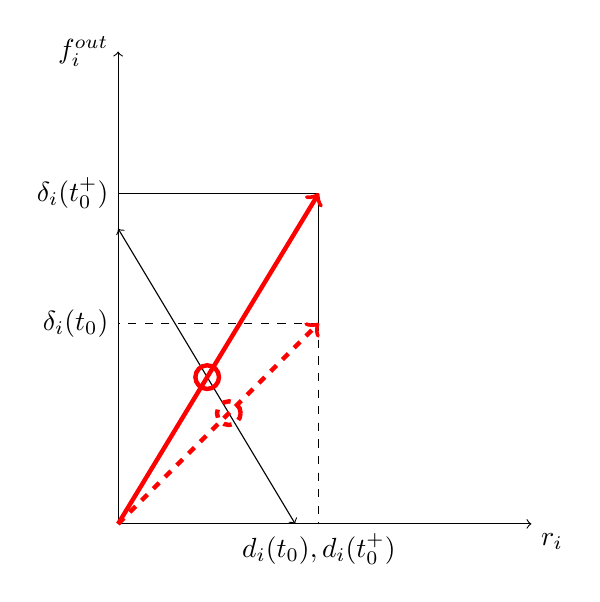
\begin{tikzpicture}[scale=\scale,domain=0:1]

\def \rampDem{1.7}
\def \rampDemPlus{1.7}
\def \dem{1.7}
\def \demPlus{2.8}
\def \priorityRat{0.6}
\def \splitRat{0.4}
\def \totalFlow{1.5}

\coordinate (Z) at (0,0);
\coordinate (I1) at (\rampDem, 0);
\coordinate (I1') at (\rampDemPlus, 0);
\coordinate (I2) at (0, \dem);
\coordinate (I2') at (0, \demPlus);
\coordinate (I3) at (\rampDem, \dem);
\coordinate (I3') at (\rampDemPlus, \demPlus);
\coordinate (A) at (0, {\totalFlow/(1-\splitRat)});
\coordinate (B) at (\totalFlow, 0);
\coordinate (C) at ({(1-\priorityRat)/\priorityRat*\dem}, \dem);
\coordinate (D) at (intersection of I2'--I3' and Z--C);


\draw[->] (Z) -- (3.5,0) node[below right]{$r_i$};
\draw[->] (Z) -- (0,4) node[left]{$f^{\text{out}}_i$};

\draw[dashed] (I3) -- (I1) node[below]{$d_i(t_0),d_i(t_0^+)$};
\draw[dashed] (I3) -- (I2) node[left]{$\delta_i(t_0)$};
\draw[dashed] (I3) -- (I1');
\draw (I3) -- (I3');
\draw (I3') -- (I2') node[left]{$\delta_i(t_0^+)$};
\draw[<->] (A) -- (B) node[yshift=1cm, xshift=0cm]{};
\draw[->, dashed, red, ultra thick] (Z) -- (I3) node[midway, xshift=1cm]{};
\draw[->, red, ultra thick] (Z) -- (I3') node[midway, xshift=1cm]{};
\draw [red, ultra thick, radius=.1, dashed] (intersection of A--B and Z--I3) circle;
\draw [red, ultra thick, radius=.1] (intersection of A--B and Z--I3') circle;

\end{tikzpicture}